


\chapter{Introduction}
\chaptermark{ Introduction}
\HRule \\[-0.5cm] % Horizontal line

\label{Chapter1} % For referencing the chapter elsewhere, use \ref{Chapter1}

\lhead{\emph{\textbf{Chapter1:} Introduction}} % This is for the header on each page - perhaps a shortened title

%----------------------------------------------------------------------------------------
%	SECTIONS
%----------------------------------------------------------------------------------------





\begin{spacing}{1.5}
\section{Multinomial Naive Bayes}

% Spoken language recognition is a task through which we verify or identify the
% language spoken (e.g. English, Hindi, Odia, Bengali etc.) in a speech sample. Spoken language recognition has numerous application in a wide range of multilingual services. Automatic routing of an incoming call to a human switchboard operator is a popular example of the automatic language recognition system. Apart from this, the spoken language recognition system can also be useful for various applications like spoken language translation, multilingual speech recognition, spoken document retrieval. It is also fruitful in intelligence and security application for information distillation~\cite{li2013spoken}. 

% Human performs the language recognition task most efficiently. With a short period of training, people are able to recognize the language within seconds of hearing an utterance, even if they are not familiar with the language they can give subjective judgment based on the similarity of the language (e.g. sounds like English). Hence, like any other artificial intelligence technologies, spoken language recognition aims to replicate such human's ability through computational means.

% In general, human use two broad classes of information, prelexical information and lexical-semantic information to discriminate one language from other~\cite{zhao2008cortical}. Acoustic phonetics, phonotactics and prosodic information of an utterance of the language, comes under prelexical information, whereas the words and syntax (i.e. grammar, Phases) level information about a language comes under lexical information. It has also investigated that infants, who have not gained a good lexical knowledge can be able to discriminate languages using prelexical information~\cite{ramus1999language}. Similarly, when an adult is dealing with two unfamiliar languages also use the prelexical information for discrimination. But when the infants' and adult's language experience increases, lexical semantic information plays a vital role for discrimination~\cite{zhao2008cortical}. Hence there is no doubt that both prelexical and lexical information contributes to the human perceptual process for spoken language recognition. While we know that it requires a major effort to get hold of the lexical information of a new language. Therefore, we can also say human rapidly use the prelexical information for the language recognition process. So, the research community paid more attention to capturing the prelexical information for the development of automatic spoken language recognition system.

% Prelexical information of a language consists of acoustic phonetics (spectrum, phone inventory), phonotactics (sequences of sounds), prosodic (duration, pitch, intonation) information~\cite{li2013spoken}. From the literature, it is shown that the prosodic cues are less informative than the phonotactic one~\cite{ramus1999language,navratil2001spoken}. Therefore, most of the works reported in the literature towards spoken language recognition use acoustic phonetics information or phonotactics information or a combination of both information for discrimination of spoken languages.  

% The human speech apparatus is capable of producing a wide range of sounds. Speech sounds as concrete acoustic events are referred to as phones. Each language has a different set of phones and even if some phones are common in some languages, but their pronunciation is different~\cite{li2013spoken}. These differences guarantee each language have different acoustic feature distribution. Therefore, people attempt to model the acoustic-phonetic distribution of a language using the acoustic features. 

% In phonological studies, it can be summarised that each language has its unique phonological rules to govern the combination of different phones. For example, the sequence of phones that occur frequently in one language could be rare in other languages. Such phonotactic constraints can be characterized by a phone n-gram model. In this approach, people try to distinguish languages by comparing the frequency of occurrence of certain reference sounds or sound sequences with that of the target language.

% In general acoustic-phonetics based spoken language recognition systems, extract acoustic features (mel frequency cepstral coefficient (MFCC), perceptual linear prediction coefficient (PLP), linear prediction cepstral coefficient (LPCC), shifted delta coefficient (SDC)) from speech utterance of each language~\cite{rabiner1993yegnanarayana,hermansky1990perceptual,torres2002approaches}, using classification techniques (shallow neural networks (NN), vector quantization (VQ), Gaussian mixture model (GMM), hidden Markov model (HMM), Gaussian mixture model and universal background model (GMM-UBM), I-Vector, Deep neural networks (DNN)) try to model the acoustic features of each language~\cite{wong2002methods,zissman1996comparison,zissman1993automatic,sugiyama1991automatic,braun1998automatic,richardson2015deep}. At the time of testing the acoustic feature of the test utterance were compared with each of the language models and the language model giving higher likely-hood score is hypothesized as the language of test utterance. In the case of phonotactic approach the phone sequence of the test utterance was compared with a global phone based n-gram model of each language and the model giving higher likelihood value is identified~\cite{jurafsky2000speech}. Though phonotactic approaches give better performance in some cases, and the combination of acoustic-phonetic and phonotactics approaches improves the overall performance, the main drawback of phonotactic approaches is that it requires the phonetic transcriptions of speech utterances which is very difficult to obtain~\cite{li2013spoken}.

% The impressive performance improvement got by using deep neural network (DNN) for automatic speech recognition motivates the research community to use various DNN architectures to perform spoken language recognition task~\cite{richardson2015deep,gonzalez2014automatic,lopez2014automatic,lopez2016use,garcia2016stacked,snyder2018spoken,sarma2018language}. DNN architectures can be used for both classification and feature extraction (bottleneck feature (BNF)). Phonetic aware DNN is also used for language recognition where the GMM posteriors are replaced by the DNN Senones for i-vector extraction~\cite{richardson2015deep}. As the spoken language discrimination ability depends on both the acoustic and phonotactic information, people try to extract features having both the information from the bottleneck layer by providing acoustic features to the input of a feed-forward DNN and posterior senone probabilities to the output of DNN~\cite{richardson2015deep}. Currently, the time delay neural network based X-vector framework is the state-of-the-art technique for spoken language recognition~\cite{snyder2018spoken,sarma2018language}. In the X-vector framework, after x-vector computation, the same classification technique like I-vector was followed.  




% \section{Language identification, Language verification and Language diarization}
% Like speaker recognition, spoken language recognition can be also be viewed as:
% \begin{itemize}
%     \item Language identification
   
%     \item Language verification
%     \item Language diarization
% \end{itemize}
 
% \subsection{Language identification and  verification}

% In language identification, the task is to determine the spoken language of the test utterance by comparison with a set of enrolled language models. The language model with which the test utterance giving higher likely-hood score is hypothesized as the language of test utterance. 
% If the language's of all the test utterance is available with the machine, then it is called Closed-set language identification, otherwise called Open-set language Identification. The performance of the language Identification system is evaluated in terms of identification accuracy.

% In the language verification, the task is to validate the test utterance in the form of target (or claimed) language or not (i.e the decision had been taken between two hypotheses). where the decision has to be made between two hypotheses with respect to a decision threshold. The basic block diagram of the language identification/ language verification system is shown in figure~\ref{lr}. 
%  \begin{figure}[h]
% \centering{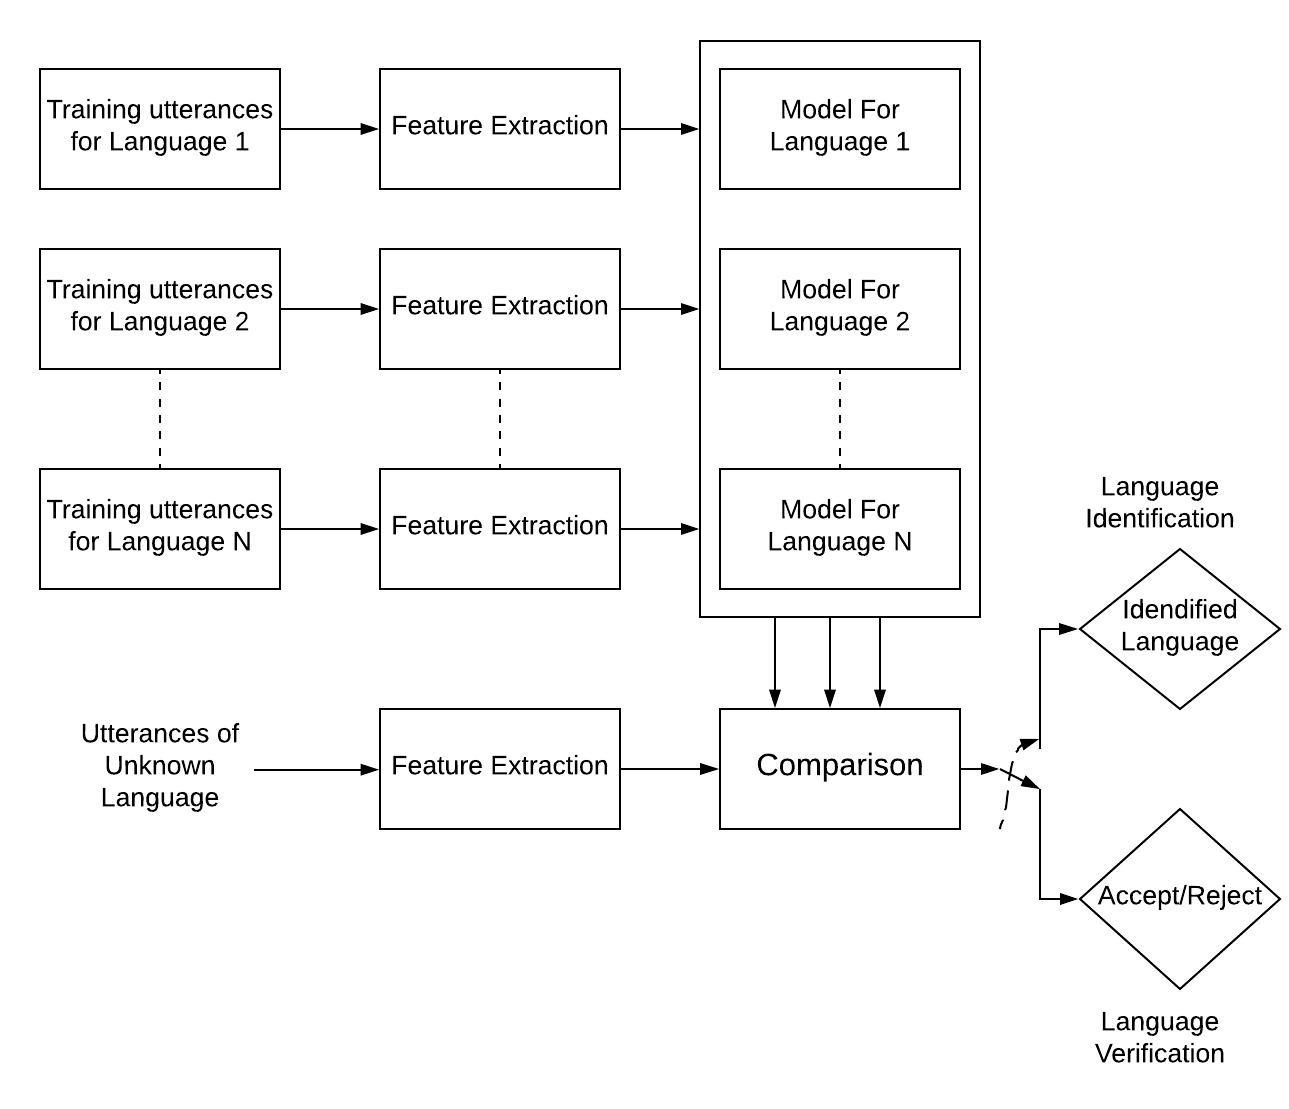
\includegraphics[scale=.65]{Images/lr.jpeg}}
% \caption{Basic block diagram of language identification/verification system.}
% \label{lr}
% \end{figure} 
  
%   Language recognition could be best manifested as a multiclass recognition problem, where the input belongs to one from the set of discrete classes. The objective is to recognize the class of the input. Let we have N target classes, $\{L_{1},L_{2},\ldots,L_{N}\}$. In the close-set there are N different specified languages, whereas in open set there are $N-1$ specified languages corresponds to $L_{1}, L_{2},\ldots, L_{N-1}$ target classes and  $L_{N}$ class denotes any unseen out of set languages. If $O$ is the spoken utterance
% \begin{itemize}
%     \item Language identification: Which of the N language does $O$ belongs to?
%     \item Language verification: Does $O$ belongs to language $L_{l}$ or to other $N-1$ languages? 
% \end{itemize}




% \subsection{Language diarization}
% Language diarization is a task to perform automatic language segmentation and recognition in a code-switched speech. Language diarization is different from language recognition, as in language recognition the test utterance is a monolingual utterance and the task is to identify the language identity. But in the case of language diarization, the test utterance's both the language identity and boundary of the language transition is unknown and the task is to find the language identity and language boundary. The basic block diagram of the language diarization system is shown in figure~\ref{ld}. The most challenging part of language diarization is the duration of mono-lingual segments of code-switched speech, which are much shorter than those traditionally studied in the language recognition. The performance of language diarization was measured in-terms of frame error rate (FER)~\cite{lyu2013language}. The application of language diarization can improve the performance of multilingual automatic speech recognition (ASR) system by improving the performance of Large vocabulary continuous speech recognition (LVCSR) when the test utterance contains code switch speech~\cite{lyu2013language}. Therefore for a country like India, where people use more than two languages while conversation, the language diarization system may play an important role to enhance the ASR performance.
 
%  \begin{figure}[h]
% \centering{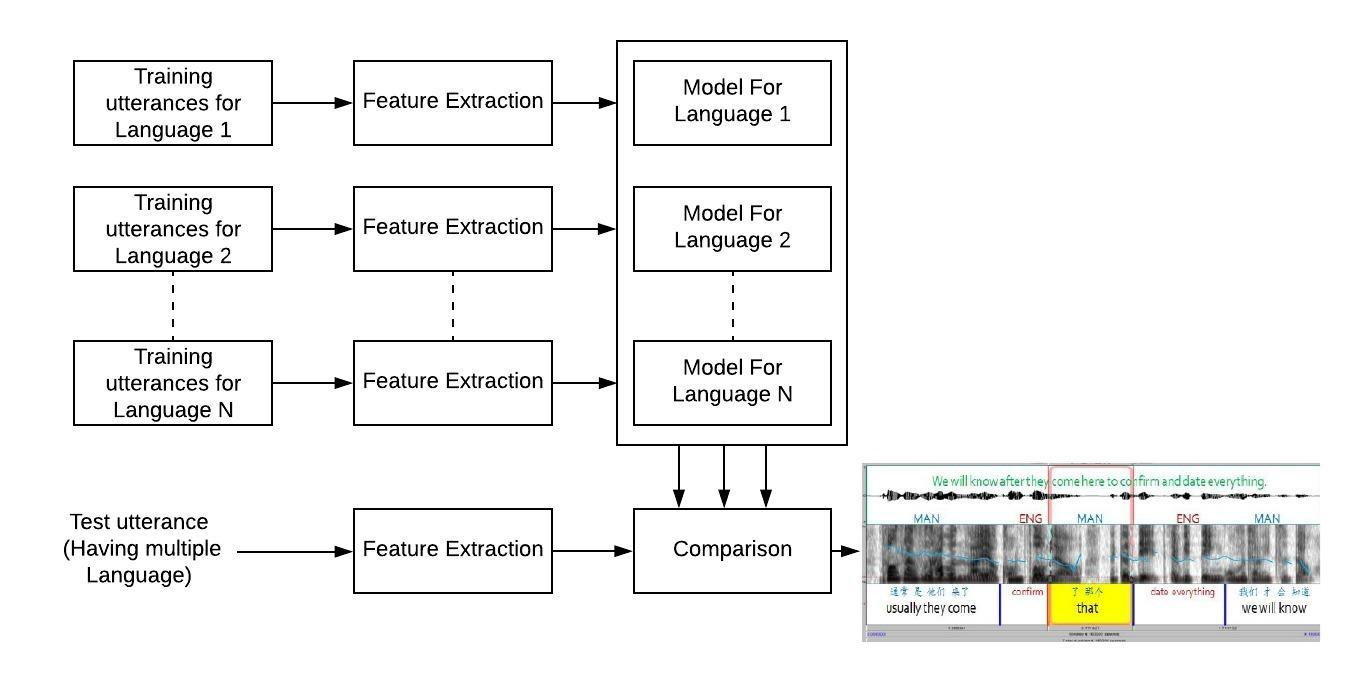
\includegraphics[scale=.65]{Images/language_diarization.jpeg}}
% \caption{Basic block diagram of language diarization system~\cite{lyu2013language1}.}
% \label{ld}
% \end{figure} 
% As like spoken language recognition, the language diarization can be performed by using both acoustic and phonotactic approach. In~\cite{lyu2013language}, Lyu et al. used 63-hour conversational South-East-Asia Mandarin/English (SEAME) code-switch corpus to perform language diarization experiment. In SEAME database, average language intervals in monolingual Mandarin and English segments are about 0.81 seconds and 0.67 seconds, respectively. The average number of language changes within a code-switched utterance is about $2.2$. They propose a phonotactic approach, where the acoustic features are passed through a phone recognizer and the phone recognizer output with different context was used to train a conditional random field (CRF) classifier. The performance of the system increases with increase in no of context frames. The best performance achieved was 14.4\% FER with context length $2$. In~\cite{yilmaz2017language}, Yilmaz et al. used an acoustic approach (BNF-UBM-I-vector) to perform language diarization. They use language diarization to perform automatic transcription of bilingual broadcast data. They observed that the use of language diarization with monolingual ASR instead of using bilingual ASR system improve the performance bilingual automatic transcription system. 
% \section{Major milestones for language recognition}
% The first attempt of identifying the spoken language was proposed in~\cite{leonard1974automatic}, where the phonotactic patterns were used to distinguish languages by computing the frequency of occurrence of certain sound units. To perform the language identification task they used five different languages and achieved an overall accuracy of 64\%. In the next attempt~\cite{house1977toward}, Markov process was used to model the sequence of sounds having a manual transcription of the utterances of eight different languages. The next attempt was coming on 1980~\cite{li1980statistical}, where they modeled the real speech data using a Markov process with broad phone classes of five different languages and obtained a testing accuracy of 80\%. 

% In 1982 Cimarusti et al.~\cite{cimarusti1982development} first time extracted acoustic features from the speech signal and modeled using a polynomial classifier. In this work they derived 100 features (i.e 15 area functions, 15 auto-correlation coefficients, 5 bandwidths, 15 Cepstral coefficients, 15 filter coefficients, 5 formant frequencies, 15 log area ratios, and 15 reflection coefficients) from the linear prediction coefficient of the speech utterance having frame size 30 msec with a context shift of 30 msec. They used 8 languages in the study and achieved an accuracy of 84\%. In~\cite{foil1986language}, Foil et al. used noisy radio recordings to identify the languages, where they examined two types of language identification systems. In the first approach, they extracted seven prosodic features (based on rhythm and intonation) from pitch and energy contour. In the second they used formant frequencies (in terms of values and locations) to represent the characteristic sound patterns of the language. A k-means clustering algorithm and VQ were used for classification. The language identification performance achieved on three languages was 64\% correct with 11\% rejection on the test data duration of 4.5 seconds with the signal to noise ratio (SNR) of 5 dB. Motivating by the work of Foil et al., In~\cite{goodman1989improved} Goodman et al. attempted to improve the LPC based format extraction algorithm with six language database and test data duration of smaller than 10 seconds. The final performance was reported in terms of, a function of time, SNR and no-decision rate. 

% In~\cite{sugiyama1991automatic}, Sugiyama et al. performed VQ classification on LPC derived features. They explored the difference between using one VQ codebook per language vs. one common VQ codebook for all languages, where the languages were classified according to their occurrence probability in histogram patterns. The experiment results show that the recognition rates for the first and second algorithms were 65\% and 80\%, respectively. The speech database used in this paper contains 20 languages: 16 sentences uttered twice by 4 males and 4 females with a duration of 8 seconds each.

% In~\cite{nakagawa1992speaker}, Nakagawa et al. compared four methods VQ, discrete HMM, continuous density HMM and GMM. Comparative analysis of all mentioned methods was conducted in four languages. In the final performance, it is shown that the results obtained using continuous HMM and GMM (81.1\%) were better than vector quantization (77.4\%) and discrete HMM (47.6\%).

% In~\cite{zissman1993automatic}, Zissman et al. perform a comparative study using HMM and GMM as a classifier with standard MFCC features along with their delta coefficients. The algorithms were evaluated on four multi-language speech databases: a three language subset of the spoken language library, a three language subset of a five-language Rome laboratory database, the 20 language CCITT database, and the ten languages OGI telephone
% speech database~\cite{muthusamy1992ogi}. They observed that performance of single state HMM (I.e. GMM) classifier is comparable with the performance of multi-state HMM. The authors mentioned that the observed result may be due to the lack of training data to train the multi-state HMM. 

% In~\cite{zissman1996comparison}, Zissman et al. compared the performance of four approaches for automatic spoken language identification. The approaches taken by them are  GMM for acoustic feature classification, single-language phone recognition followed by language-dependent interpolated n-gram language modeling (PRLM), parallel PRLM (which uses multiple single-language phone recognizer, each trained in a different language), and language dependent parallel phone recognition (PPR). The approaches were evaluated with the OGI multi-language telephone speech corpus and NIST 1994 corpus. They observed the systems have phone recognizer performed better than the GMM classifier. The top-performing system was parallel PRLM, which exhibited an error rate of 2\% for 45-s utterances and 5\% for 10-s utterances in two-language, closed-set, forced choice
% classification. The error rate for 11-language, closed-set, forced-choice classification was 11\% for 45-s utterances and 21\% for 10-second utterances.

% In~\cite{wong2002methods}, the authors used GMM-universal background model (UBM) classifier in the spoken language recognition task, by motivating the performance of GMM-UBM over standard GMM in speaker recognition~\cite{reynolds2000speaker}. They used 39 dimensions MFCC features along with its velocity and acceleration coefficients with vocal tract length normalization (usually use to suppress speaker dependent information). They used GMM-UBM classifier, to model the acoustic feature vectors. They observed the performance of GMM-UBM is better (i.e 13.4\%) than Parallel PRLM approach (i.e 16.6\%) in case of 45 sec testing case, but in the case of 10 sec testing case the performance of parallel PRLM (PPRLM) (i.e 24.8\%) is better than the GMM-UBM based approach (i.e 27\%). The overall fused system performance is 10.2\% for 45 sec and 18.4\% for the 10-sec testing case. They used OGI Multi-Language Telephone Speech Corpus and NIST 1994 corpus for conducting experiments.

% In~\cite{torres2002approaches}, they were motivated by the performance of multiple-language phone recognition and n-gram language modeling on language identification task, which indicates that the automatic language identification task largely depends on the sequence information of speech utterances. The standard MFCC features are not able to capture sequence information of the utterances. In this paper they used shifted delta coefficient (SDC) which captured sequence information of speech utterances. They observed that the results obtained are comparable with phonotactic based PPRLM method. They used CallFriend and OGI corpora for system evaluation and achieved the best performance of 6.90\% in CallFriend corpora.


% In~\cite{li2007vector}, they proposed a vector space modeling (VSM) method for automatic spoken language identification (LID) by motivating that the overall sound characteristics of all spoken languages can be covered by a universal collection of acoustic units, which can be characterized by the acoustic segment models (ASMs). A spoken utterance is then decoded into a sequence of ASM units. The ASM framework furthers the idea of language-independent phone models for LID by introducing an unsupervised learning procedure to circumvent the need for phonetic transcription. This is analogous to representing a text document as a term vector.  They converted a spoken utterance into a feature vector with its attributes representing the co-occurrence statistics of the acoustic units, then built a vector space classifier for LID. The proposed VSM approach leads to a discriminative classifier at the back-end. The observed result tells that the latter approach gives superior performance over likelihood-based n-gram language modeling (LM) back-end for long utterances. The performance of the proposed VSM framework in-terms of equal error rate (EER) was 2.75\% and 4.02\% in the 1996 and 2003 NIST language recognition evaluation (NIST-LRE) 30-second tasks, respectively.

% In~\cite{ma2007spoken}, they used an ensemble of binary classifiers with shifted delta coefficient (SDC) to perform spoken language recognition. They adopted a distributed output coding strategy in ensemble classifier design, where they decomposed a multiclass language recognition problem into many binary classification tasks, each of which addresses a language recognition sub-task by using a component classifier. Then, they combined the results of the component classifiers to form an output code as a hypothesized solution to the overall language recognition problem. In this way, they effectively projected the high-dimensional feature vectors into a low-dimensional space by maintaining language discriminating characteristics of the spoken utterances. By fusing the output codes from both phonotactic features and cepstral features, they achieved an equal-error-rates of 1.38\% and 3.20\% for 30-second trials on the 2003 and 2005 NIST-LRE databases respectively.



% In~\cite{dehak2011language}, motivated by the improvement in performance of speaker recognition system using I-vector based modeling, the authors use I-vector based modeling approach in spoken language recognition task. They achieved a performance of 2.1\% EER on NIST 2009 evaluation protocol.

% In~\cite{song2013vector}, i-vector representation based on BNF features is presented for language identification (LID). In the proposed system, the BNF features are extracted from a deep neural network, which can effectively mine the contextual information embedded in speech frames. The i-vector representation of each utterance is then obtained by applying a total variability approach to the BNF features. The resulting performance of the LID has been significantly improved with the proposed BNF feature based i-vector representation. The obtained best result was 1.98\%, 3.47\%, 9.71\% in-terms of EER  on the NIST 2009 evaluation set with 30, 10 and 3 seconds test duration respectively.

% In~\cite{gonzalez2014automatic}, they explore the use of Long Short-Term Memory (LSTM) recurrent neural networks (RNNs) for automatic language identification (LID). The use of RNNs is motivated by their better ability in modeling sequences with respect to feedforward networks. From the work, it is observed that long short term memory (LSTM) RNNs can effectively exploit temporal dependencies in acoustic data and learn relevant features for language discrimination. The proposed approach is compared to baseline i-vector and feedforward Deep Neural Network (DNN) systems in the NIST Language Recognition Evaluation 2009 dataset. The work shows LSTM RNNs achieve better performance than feedforward net based DNN system and i-vector system. The performance using LSTM RNN was 8.35\% in terms of average EER with 3-second test data, which is better compared to 9.58\% in feedforward net with 8 layers and 15.89\% in I-vector system. 

% In~\cite{lei2014application}, they used a convolutional neural network (CNN) for the training of automatic speech recognition (ASR) system, the posterior of the model is used for i-vector extraction instead of UBM posteriors. The task was performed on the RATS database with five target languages (Farsi, Urdu, Pashto, Arabic, Levantine, and Dari) and achieved a performance of 10.95\%, 5.24\% and 3.53\% with 30, 10 and 3 seconds test utterances respectively. 

% In~\cite{richardson2015deep}, Richardson et al. compared standard i-vector and various deep learning approaches for spoken language recognition task. Motivated by the gain of performance in ASR by using deep learning frameworks, the authors used deep feedforward network as a classifier, phonetic aware deep feedforward network for i-vector computation and bottleneck features were extracted from a deep feedforward network, which is used later to model the i-vector. Finally, it is observed that the performances of bottleneck feature (BNF) based i-vector system outperform the performances of all other systems. In NIST 2011 language recognition evaluation set the best performance achieved in-terms of $C_{avg}$ was 0.304\% using DNN as posterior in 30 seconds, 1.24\% in 10 seconds and 7.53\% in 3 seconds using GMM as posterior with BNF-i-vector system.     


% In~\cite{zhang2018language}, Zhang et al. mentioned that traditional bottleneck feature extraction requires additional transcribed speech information, which is very difficult to get. Hence they proposed alternate unsupervised deep learning methods for bottleneck feature extraction. They used unsupervised cluster Gaussian mixtures for posterior labeling of frames instead of using posterior phone labeling for bottleneck feature extraction. They also used variational autoencoder and adversarial autoencoder for speech feature extraction. Then they used the i-vector framework to classify spoken languages. In this work they use three databases: 1) a four Chinese dialect dataset, 2) a five Arabic dialect corpus, and 3) multigenre broadcast challenge corpus (MGB-3) for language recognition task. The best fusion system performance archived in Chinese dataset was 95.7\% accuracy, in Pan-Arabic was 81.3\% accuracy and in MGB-3 dataset was 65.4\% accuracy.

% In~\cite{snyder2018spoken}, Snyder et al. applied x-vectors to the task of spoken language recognition motivated by the performance of x-vector in the speaker recognition task. The x-vector framework consists of a deep neural network that maps sequences of speech features to fixed-dimensional embeddings, called x-vectors. In this framework, long-term language characteristics are captured in the network by a temporal pooling layer that aggregates information across time. Once x-vectors were computed, the same classification procedure like i-vectors was followed. In 2017 NIST-LRE, x-vectors outperformed all state-of-the-art i-vector systems. The best performance achieved using x-vectors (multilingual BNF with augmentation) in terms of $c_{avg}$ was 14.0\% in 3 seconds of test data.

% The summary of all the works reported above towards spoken language recognition is tabulated in table~\ref{tab_review} and table~\ref{tab_review2}.

% \begin{table}
% \caption{A summary on different studies made on language recognition.}
% \label{tab_review}
% \begin{tabular}{|l|l|l|l|}
% \hline
% LRE Systems         & Method used                                                                                          & Performance                                                                                                                 & Database                                                                                                \\ \hline
% Leonard et al.~\cite{leonard1974automatic}      & Phonotactic Pattern                                                                                  & \begin{tabular}[c]{@{}l@{}}Identification \\ accuracy=64\%\end{tabular}                                                     & \begin{tabular}[c]{@{}l@{}}In house data \\ (five language)\end{tabular}                                \\ \hline
% House et al.~\cite{house1977toward}        & \begin{tabular}[c]{@{}l@{}}Markov Process\\ (Manual phone\\ transcription)\end{tabular}              &                                                                                                                             & \begin{tabular}[c]{@{}l@{}}In house data\\ (Eight language)\end{tabular}                                \\ \hline
% Li et al.~\cite{li1980statistical}           & \begin{tabular}[c]{@{}l@{}}Markov Process\\ (Real speech model)\end{tabular}                         & \begin{tabular}[c]{@{}l@{}}Identification \\ accuracy=80\%\end{tabular}                                                     & \begin{tabular}[c]{@{}l@{}}In house data \\ (Five language)\end{tabular}                                \\ \hline
% Cimarusti et al.~\cite{cimarusti1982development}    & \begin{tabular}[c]{@{}l@{}}100 dimension \\ acoustic feature\\ (Polynomial Classifier)\end{tabular} & \begin{tabular}[c]{@{}l@{}}Identification \\ accuracy=84\%\end{tabular}                                                     & \begin{tabular}[c]{@{}l@{}}In house data\\ (Eight language)\end{tabular}                                \\ \hline

% Foil et. al.~\cite{foil1986language}        & \begin{tabular}[c]{@{}l@{}}Prosodic feature,\\ Frequency of\\ Format location\end{tabular}           & \begin{tabular}[c]{@{}l@{}}Identification \\ accuracy=64\%\end{tabular}                                                     & \begin{tabular}[c]{@{}l@{}}In house data,\\ Noisy data\\ with 5 dB SNR\\ (Three language)\end{tabular} \\ \hline
% Goodman et al.~\cite{goodman1989improved}      & \begin{tabular}[c]{@{}l@{}}Improved LPC based\\ Format extraction\\ algorithm\end{tabular}          &                                                                                                                             & \begin{tabular}[c]{@{}l@{}}In house data,\\ Noisy data\\ (Six language)\end{tabular}                   \\ \hline
% Sugiyama et al.~\cite{sugiyama1991automatic}     & \begin{tabular}[c]{@{}l@{}}LPC derive feature\\ VQ Code-book\end{tabular}                             & \begin{tabular}[c]{@{}l@{}}Identification \\ accuracy=80\%\end{tabular}                                                     & \begin{tabular}[c]{@{}l@{}}In house data,\\ (Twenty language)\end{tabular}                              \\ \hline
% Nakagawa et al.~\cite{nakagawa1992speaker}    & \begin{tabular}[c]{@{}l@{}}VQ,\\ Discrete HMM,\\ Continuous HMM,\\ GMM\end{tabular}                  & \begin{tabular}[c]{@{}l@{}}Identification \\ accuracy=81.1\%\end{tabular}                                                   & \begin{tabular}[c]{@{}l@{}}In house data,\\ (Four language)\end{tabular}                                \\ \hline
% Zissman et al.~\cite{zissman1993automatic}     & \begin{tabular}[c]{@{}l@{}}HMM,\\ GMM\\ (MFCC+ Delta)\end{tabular}                                   &                                                                               \begin{tabular}[c]{@{}l@{}}Identification \\ accuracy=80\%\end{tabular}                                              & OGI-11L Data set                                                                                        \\ \hline
% Zissman et al.~\cite{zissman1996comparison}      & \begin{tabular}[c]{@{}l@{}}GMM\\ Parallel PRLM\end{tabular}                                          & \begin{tabular}[c]{@{}l@{}}Error rate\\ 45 sec- 11\%\\ 10 sec- 21\%\end{tabular}                                            & \begin{tabular}[c]{@{}l@{}}OGI-11L Data set\\ NIST 1994\end{tabular}                                                                                                                                   \\ \hline
% Wong et al. ~\cite{wong2002methods}         & GMM-UBM                                                                                              & \begin{tabular}[c]{@{}l@{}}Error rate\\ 45 sec- 10.2\%\\ 10 sec- 18.4\%\end{tabular}                                        & \begin{tabular}[c]{@{}l@{}}OGI-11L Data set\\ NIST 1994\end{tabular}                                    \\ \hline
% Carrasquillo et al.~\cite{torres2002approaches} & \begin{tabular}[c]{@{}l@{}}SDC-GMM,\\ PPRLM\end{tabular}                                             & \begin{tabular}[c]{@{}l@{}}Error rate\\ 45 sec- 6.90\%\end{tabular}                                                         & \begin{tabular}[c]{@{}l@{}}OGI  Data set\\ CallFriend Corpus\end{tabular}                               \\ \hline
% Li et al.~\cite{li2007vector}           & \begin{tabular}[c]{@{}l@{}}Vector Space\\ Modelling (VSM)\end{tabular}                               & \begin{tabular}[c]{@{}l@{}}EER\\ 30 sec- 2.75\% (1996)\\ 30 sec- 4.02\% (2003)\end{tabular}                                 & \begin{tabular}[c]{@{}l@{}}NIST-1996\\ NIST-2003\end{tabular}                                           \\ \hline


% \end{tabular}
% \end{table}



% \begin{table}[ht]
% \caption{A summary on different studies made on language recognition.}
% \label{tab_review2}
% \begin{tabular}{|l|l|l|l|}
% \hline
% LRE Systems         & Method used                                                                                          & Performance     & Database    \\ \hline
%   Ma et al.~\cite{ma2007spoken}           & \begin{tabular}[c]{@{}l@{}}SDC\\ Binary Classification\end{tabular}                                   & \begin{tabular}[c]{@{}l@{}}EER\\ 30 sec- 1.38\% (2003)\\ 30 sec- 3.20\% (2005)\end{tabular}                                 & \begin{tabular}[c]{@{}l@{}}NIST-2003\\ NIST-2005\end{tabular}  \\ \hline                                                                                                       
                                         
% Dehak et al.~\cite{dehak2011language}        & I-vector                                                                                             & \begin{tabular}[c]{@{}l@{}}EER\\ 30 sec-2.1\%\end{tabular}                                                                  & NIST-2009                                                                                               \\ \hline
% Song et al.~\cite{song2013vector}         & BNF-I vector                                                                                         & \begin{tabular}[c]{@{}l@{}}EER\\ 30 sec-1.98\%\\ 10 sec-3.47\%\\ 3 sec-9.71\%\end{tabular}                                  & NIST-2009                                                                                               \\ \hline
% Gonzalez et al.~\cite{gonzalez2014automatic}     & RNN-LSTM                                                                                             & \begin{tabular}[c]{@{}l@{}}EER\\ 3 sec- 8.35\%\end{tabular}                                                                 & NIST-2009                                                                                               \\ \hline
% Lei et al.~\cite{lei2014application}          & CNN-I vector                                                                                         & \begin{tabular}[c]{@{}l@{}}EER\\ 30 sec- 10.95\%\\ 10 sec- 5.24\%\\ 3 sec-3.53\%\end{tabular}                               & \begin{tabular}[c]{@{}l@{}}RATS\\ (Five language)\end{tabular}                                          \\ \hline


% Richardson et al.~\cite{richardson2015deep}   & \begin{tabular}[c]{@{}l@{}}DNN\\ DNN-I-Vector\\ BNF-UBM-I-vector\\ BNF-DNN-I-vector\end{tabular}       & \begin{tabular}[c]{@{}l@{}}$C_{avg}$\\ 30 sec-0.304\%\\ 10 sec-1.24\%\\ 3 sec- 7.53\%\end{tabular}                               & NIST-2011                                                                                               \\ \hline
% Zhang et al.~\cite{zhang2018language}        & \begin{tabular}[c]{@{}l@{}}Unsupervised BNF\\ Autoencoder Feature\end{tabular}                       & \begin{tabular}[c]{@{}l@{}}Identification\\ accuracy\\ Chinese - 95.7\%\\ Pan Arabic - 81.3\%\\ MGB-3 - 65.4\%\end{tabular} & \begin{tabular}[c]{@{}l@{}}Chinese Dialect\\ Pan Arabic\\ MGB-3\end{tabular}                           \\ \hline
% Snyder et al.~\cite{snyder2018spoken}       & X-vector                                                                                             & \begin{tabular}[c]{@{}l@{}}$C_{avg}$\\ 3 sec - 14.0\%\end{tabular}                                                             & NIST-2017                                                                                               \\ \hline

% \end{tabular}
% \end{table}


% \section{Databases for spoken language recognition}
% The availability of large dataset has been the major driving factor in the development of speech technology~\cite{li2013spoken}. To design a spoken language recognition system, we need a set of speech data of different languages having variations within the language like intersession variability, speaker variation, device variation and recording environment variation. 

% There are three standard organizations, who develop standard challenge databases for language recognition study. These standard corpora are Oregon graduate institute telephone speech corpus(OGI-TS), LDC call friend telephone speech corpus and NIST Language recognition corpus.

% \subsection{Oregon graduate institute telephone speech corpus (OGI-TS)}
% The OGI-TS is the first publicly available multi-lingual speech corpus developed to perform spoken Language recognition task~\cite{muthusamy1992ogi}. The OGI-TS speech corpus contains the speech from 11 languages: English, Farsi, French, German, Hindi, Japanese, Korean, Mandarin, Chinese, Spanish, Tamil, and Vietnamese. Each language contains the speech from about 80 native speakers, where each speech utterance in the corpus was spoken by a unique speaker over the telephone channel with a sampling frequency of 8kHz. The corpus was collected and developed in 1992, and the latest version was released in 2002 which includes recorded utterances from about 2052 speakers, for a total of about 38.5 hours of speech.
% \subsubsection{OGI-TS 22 language corpus}
% The current version of the OGI 22 Language corpus consists of telephone speech from 21 languages: Arabic, Cantonese, Czech, English, Farsi, German, Hindi, Hungarian, Japanese, Korean, Indonesian, Mandarin Chinese, Italian, Polish, Portuguese, Russian, Spanish, Swedish, Swahili, Tamil and Vietnamese~\cite{lander1995ogi}. The corpus contains fixed vocabulary utterances (e.g. days of the week) as well as fluent continuous speech. Approximately 20,000 utterances in 16 languages have corresponding orthographic transcriptions.


% \subsection{LDC callfriend telephone speech corpus}
% The call friend corpus released by LDC having unscripted conversion speech of 12 languages~\cite{ambikairajah2011language,li2013spoken}. These 12 languages are Egyptian Arabic, English, Farsi, French, German, Hindi, Japanese, Korean, Mandarin, Spanish, Tamil, and Vietnamese. From the 12 languages, 3 languages each having two dialects: English (American English with southern and non-southern dialect ), Mandarin (Mainland and Taiwan dialect), Spanish (Spanish-Caribbean and Spanish-Non Caribbean dialect). Dialect means the variation in utterances of the same language by the speakers belongs to the different geographical region. The database consists of 60 telephone conversations for each language, where 20 are used for the training set, 20 for the development set and 20 for the evaluation set. As per the protocol the training set is used to train the language model and classifier, the development set to train the back-end classifier and the evaluation set for final system evaluation.   
% \subsection{NIST Language recognition corpus (NIST LRE)}
% The National Institute of Standards and Technology (NIST) has conducted a series of evaluations of spoken language recognition in 1996, 2003, 2005, 2007, 2009, 2011, 2015 and 2017~\cite{martin2003nist,martin2009,greenberg20122011}.These  evaluations  have  been designed  to  foster  research progress, with the goals of
% \begin{enumerate}
%     \item Exploring promising new ideas in language recognition.
%     \item Developing advanced technology incorporating these ideas.
%     \item Measuring the performance of this technology.
% \end{enumerate}
% It has been seen that more languages are added from year to year. The emphasis of NIST LRE has been on conversational telephone speech (CTS), since most of the likely applications of the technology involve signals recorded from the public telephone system. In order to collect speech data of more languages in a cost-effective way, NIST has adopted broadcast narrow-band speech (BNBS) lately in LRE 2009, LRE 2011, LRE 2015 and LRE 2017. BNBS data are excerpts of call-in telephone speech embedded in broadcast and webcast. The call-in excerpts are used as we could expect them to cover as many speakers as possible. Broadcast entities like the Voice of America (VOA) broadcast are having more than 45 languages. Alternatively, the British Broadcast Company (BBC) also produces and distributes programs in a large number of languages. The number of target languages in NIST 1996 has 12, NIST 2003 has 12, NIST 2005 has 9, NIST 2007 has 24 with 5 open-set languages, NIST 2009 has 23 with 16 open-set languages, NIST 2011 has 24, NIST 2015 has 20 and NIST 2017 has 14. In NIST 2017, unlike previous  LREs the evaluation data will be divided into partitions based on the data source, i.e., MLS14 and VAST, for each language, resulting in a total of 28 partitions. The NIST evaluation protocol has three testing conditions:
% 30 seconds, 10 seconds and 3 seconds.

% \section{Performance measure for language recognition}

% The spoken language recognition experiments generally evaluated by identification accuracy, average equal error rate, and average detection cost~\cite{li2013spoken}.

% \subsection{Average detection cost($C_{avg}$)}
% As per NIST LRE, the language recognition system performance is evaluated in terms of average detection cost. In spoken language recognition, the
% performance is evaluated by presenting the system with a set of trials, each consisting of a test segment and a hypothesized target language. The system has to decide for each trail that whether the target language was spoken in the given segment.

% Let $N_{T}$ be the number of test segments and $N$ be the number of target languages. By presenting each test segment against all target languages, there are $N_{T}$ number of trials for each target and the system under evaluation should produce $N \times N_{T}$ number of true or false
% decisions. The average detection cost can be written as,
% $$C_{avg}=\frac{1}{N}\sum_{l=1}^{N}C_{DET}(L_{l})$$
% where $C_{DET}(L_{l})$ is the detection cost for the subset of $N_{T}$ trials for which the target language is $L_{l}$.
% $$C_{DET}(L_{l})=C_{miss}P_{tar}P_{miss}(L_{l})+C_{fa}(1-P_{tar})\frac{1}{N-1}\sum_{m \neq l}P_{fa}(L_{l},L_{m})$$

% where $C_{miss}$ and $C_{fa}$ are the cost of making false rejection (miss probability) and false acceptance. $P_{tar}$ is the prior probability of the target. In general $C_{miss}$, $C_{fa}$ and $P_{tar}$ are fixed to 1, 1 and 0.5 respectively. $P_{miss}$ is the false rejection probability and  $P_{fa}$ is the false acceptance probability. 





% \section{Summery and Discussion}
% The various key aspects of Automatic Language Recognition system are discussed in this report. It includes several key aspects of language recognition, covering language characterization and various modeling techniques useful in automatic language recognition. Various system development strategies regarding the task are also discussed. It has been seen from the literature that tremendous development is observed in language recognition in the last few decades. Incorporation of DNN technique in the field of language recognition dramatically change the performance of the system. Though the language recognition is still far from perfect. From the literature, it is observed that SDC features have better language discrimination ability than all the other available features. As SDC feature capture speech dynamics over a wide range of speech frames, which helps to capture some phonotactic information also. Before the incorporation of DNN based frameworks, SDC with i-vector framework was the state-of-art language recognition technique. After neural network based approaches evolved in the field of language recognition BNF based i-vector approach has been used as the state-of-the-art approach. Recently found that the x-vector framework, which was originally developed for speaker recognition, outperformed several state-of-the-art i-vector systems on the NIST LRE 2017 database in the language recognition task. The NIST LRE database series is the most widely used dataset for language recognition study.

% It had been shown that acoustic and phonotactic features have been widely used in the language recognition task. Whereas human listening experiments indicated that prosodic and other high-level features are equally informative. This prompts us to develop some techniques for language recognition in the future, which can effectively capture such high-level information to further improve the performance of the system.





% %\section{Background}
% % \lettrine[lines=1]{\textbf{I}}{ntroduction} Introduction
% % 
% % \section{Section 1}
% % "Section Description" ~\cite{Cite01}, "Section Description"
% % \begin{equation}
% % \label{eq1}
% % x = y + z
% % \end{equation}
% % 
% % Equation \ref{eq1} adds 2 numbers.
% % 
% % 
% % \section{Section 2}
% % "Section Description"
\end{spacing} 